\documentclass[a4paper,12pt]{article}
\fontsize{14pt}{16pt}\selectfont

% Packages
\usepackage[utf8]{inputenc}

\usepackage{graphicx}
\usepackage{microtype}
\usepackage{hyperref}
\usepackage{amsmath}
\usepackage{amsfonts}
\usepackage{fancyhdr}
\usepackage{geometry}
\usepackage{tcolorbox}
\usepackage{enumitem}
\usepackage{titlesec}  % Title spacing control
\usepackage{xcolor}
\usepackage{tikz}
\usepackage{background}  % For background image
\usepackage{eso-pic}   % add this to preamble

% Use Times Roman font for text and math
\usepackage{mathptmx}  % Times font for both text and math

% Page Layout
\geometry{top=1in, bottom=.75in, left=1in, right=1in}

% Custom Header and Footer
\pagestyle{fancy}
\fancyhead[L]{}
\fancyhead[C]{}
\fancyhead[R]{}
\fancyfoot[L]{}
\fancyfoot[C]{%
  
\begin{tikzpicture}[baseline=(base.base)]
    \node[draw, circle, inner sep=2pt, minimum size=1.2em, line width=0.3pt] (base) {\thepage};
  \end{tikzpicture}%
}
\fancyfoot[R]{}
\renewcommand{\headrulewidth}{0pt}    % Thickness of the header line
\renewcommand{\footrulewidth}{0pt}    % Footer line thickness

% Section Styling
\titlespacing*{\section}{0pt}{1ex}{1ex}
\titlespacing*{\subsection}{0pt}{1ex}{1ex}
\titlespacing*{\subsubsection}{0pt}{1ex}{1ex}
\titleformat{\section}
{\normalfont\Large\bfseries}   % format: font for the whole heading
{\thesection.}                  % label (the "1")
{0.2em}                        % horizontal sep (change this value)
{}                             % before-code
\titleformat{\subsection}
{\normalfont\large\bfseries}   % format: font for the whole heading
{\thesubsection}               % label (the "1.1")
{0.5em}                        % horizontal sep (change this value)
{}                             % before-code

\setcounter{secnumdepth}{3}  % Numbering for subsubsections
\setcounter{tocdepth}{3}      % Include subsubsections in the TOC

% Background image setup for inner pages (not the cover or end page)
\backgroundsetup{
  scale=1,
  color=black,
  opacity=1,
  angle=0,
  position=current page.south,
  vshift=14.9cm,   % Remove any vertical shift for background image
  hshift=0cm,
  contents={
\includegraphics[width=\paperwidth,height=\paperheight]{img/common/Innerfront.png}} % Path to the image
}

% Ensure text is not justified
\raggedright

\begin{document}
% ================= COVER PAGE (Full bleed, no extra blank page) =================
\clearpage
\thispagestyle{empty}

% Temporarily disable the background package for this page only
\backgroundsetup{contents={}}

% Use eso-pic for clean full-page image (recommended for covers)
\AddToShipoutPictureBG*{%
  \AtPageLowerLeft{%
    
\includegraphics[width=\paperwidth,height=\paperheight]{img/common/Cover.png}%
  }%
}

% Empty page content (just to ship the page)
\null
\clearpage

% Restore normal inner page background for the rest of the document
\backgroundsetup{
  scale=1,
  color=black,
  opacity=1,
  angle=0,
  position=current page.south,
  vshift=14.9cm,
  hshift=0cm,
  contents={
\includegraphics[width=\paperwidth,height=\paperheight]{img/common/Innerfront.png}}
}
\clearpage

% Table of Contents
\tableofcontents
\clearpage

% ================= INNER CHAPTERS =================
\section{Dashboard Overview}

The dashboard will come here

\newpage
\section{User Login and Access}
The \textbf{Telecom Monitoring System (TMS)} is an internal web-based platform designed for monitoring telecom operations, including traffic, revenue, and Quality of Service (QoS) insights. This system is accessible only within the organizational intranet environment and is intended for authorized personnel.

The platform provides a centralized dashboard to ensure efficient monitoring, reporting, and operational visibility for telecom regulatory and operational activities.

\subsection{Access Link}
To access the TMS, users must connect to the intranet and navigate to the following URL:
\begin{center}
  \texttt{https://192.168.10.20/tms-4/prod1.1/}
\end{center}
This URL is only accessible from within the organization's network. Users must ensure they are connected to the intranet to access the login page.
\subsection{Access Information}
\begin{itemize}[label=--]
  \item The system is accessible \textbf{only via NOC room intranet}.
  \item Users must have \textbf{authorized credentials} to log in.
  \item Unauthorized access is strictly prohibited.
\end{itemize}

\subsection{User Registration}
\begin{tcolorbox}[colback=yellow!10]
  \textbf{Important Notice:} User registration is \textbf{not self-service}.

  % User registration is \textbf{not self-service}.\\
  \textbf{For new user account creation, please contact:}
  {TMS NOC Room Administrator.}
\end{tcolorbox}
Provide the following details:
\begin{itemize}
  \item[\boxed{$\checkmark$}] Full Name
  \item[\boxed{$\checkmark$}] Official Designation
  \item[\boxed{$\checkmark$}] Department
  \item[\boxed{$\checkmark$}] Official Email Address
  \item[\boxed{$\checkmark$}] Contact Number
\end{itemize}
The administrator will create and provide login credentials after verification.
\newpage

\subsection{Login Instructions}
\begin{figure}[htbp]
  \centering
  \itshape
  % Replace the path below with your actual image path
  \setlength{\fboxrule}{1pt}  % Border thickness
  \setlength{\fboxsep}{3pt}   % Space between image and border
  % \framebox[0.8\linewidth]{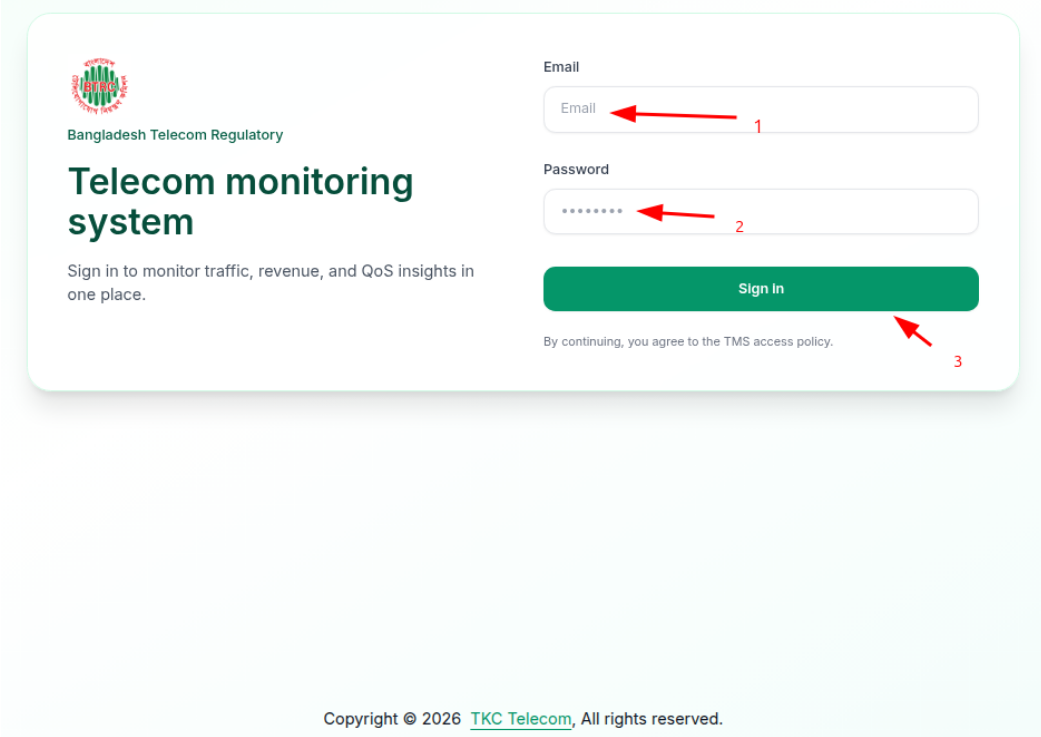
\includegraphics[width=0.8\linewidth]{img/login/login.png}}
  \colorbox{gray!20}{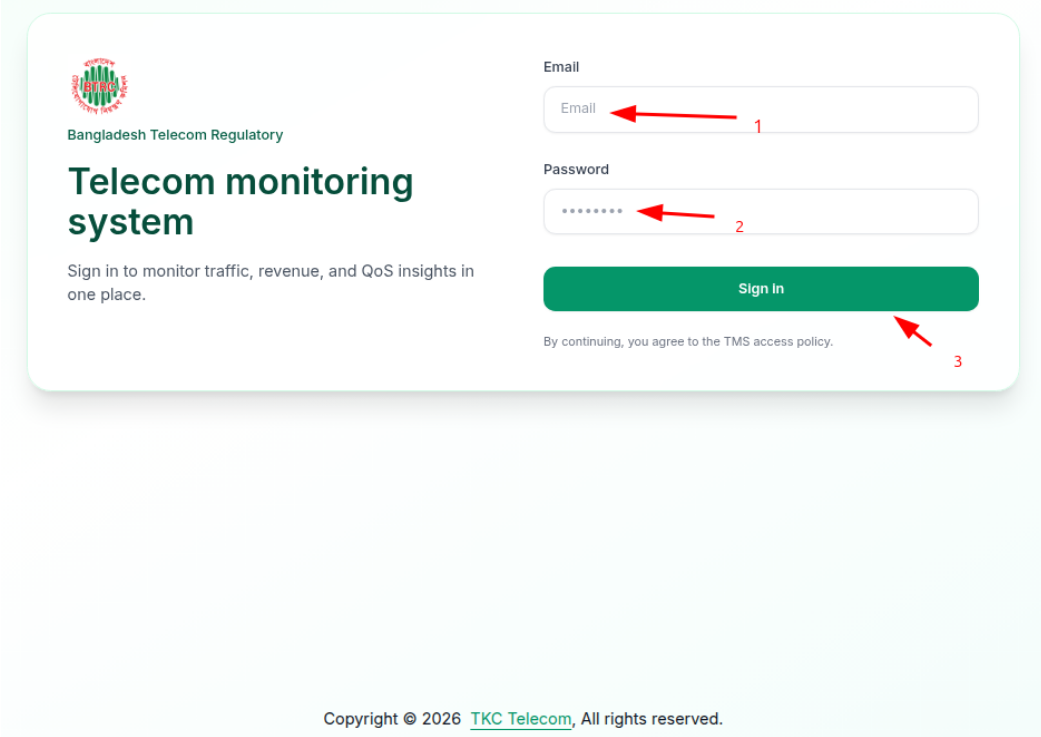
\includegraphics[width=0.8\linewidth]{img/login/login.png}}
  \caption{user login}

\end{figure}

To access the system:
\begin{enumerate}[label=\textbf{\arabic*.}]
  \item \textbf{Enter Email:} Input your \textbf{registered official email address} in the Email field.
  \item \textbf{Enter Password:} Enter your \textbf{assigned password} securely.
  \item \textbf{Sign In:} Click on the \textbf{“Sign In”} button to access the system dashboard.
\end{enumerate}

\subsection{Disclaimer}
This system is the property of the organization and is intended strictly for \textbf{authorized users only}.

\begin{itemize}[label=--]
  \item All activities performed within the system are \textbf{monitored and logged}.
  \item Unauthorized access, misuse, or data manipulation is strictly prohibited and may result in \textbf{disciplinary and legal action}.
  \item Users are responsible for maintaining the confidentiality of their login credentials.
  \item The organization reserves the right to \textbf{restrict or revoke access} at any time without prior notice.
\end{itemize}

By logging into the system, you acknowledge and agree to comply with all applicable policies, security guidelines, and regulatory requirements.

\vspace{0.5em}
\subsection{Security Guidelines}
\begin{itemize}[label=--]
  \item Do not share your password with anyone.
  \item Always log out after completing your session.
  \item Report suspicious activities immediately to the \texttt{TMS NOC Team}.
  \item Use strong passwords and update them periodically.
\end{itemize}

% ================= COVER PAGE (Full bleed, no extra blank page) =================
\clearpage
\thispagestyle{empty}

% Temporarily disable the background package for this page only
\backgroundsetup{contents={}}

% Use eso-pic for clean full-page image (recommended for covers)
\AddToShipoutPictureBG*{%
  \AtPageLowerLeft{%
    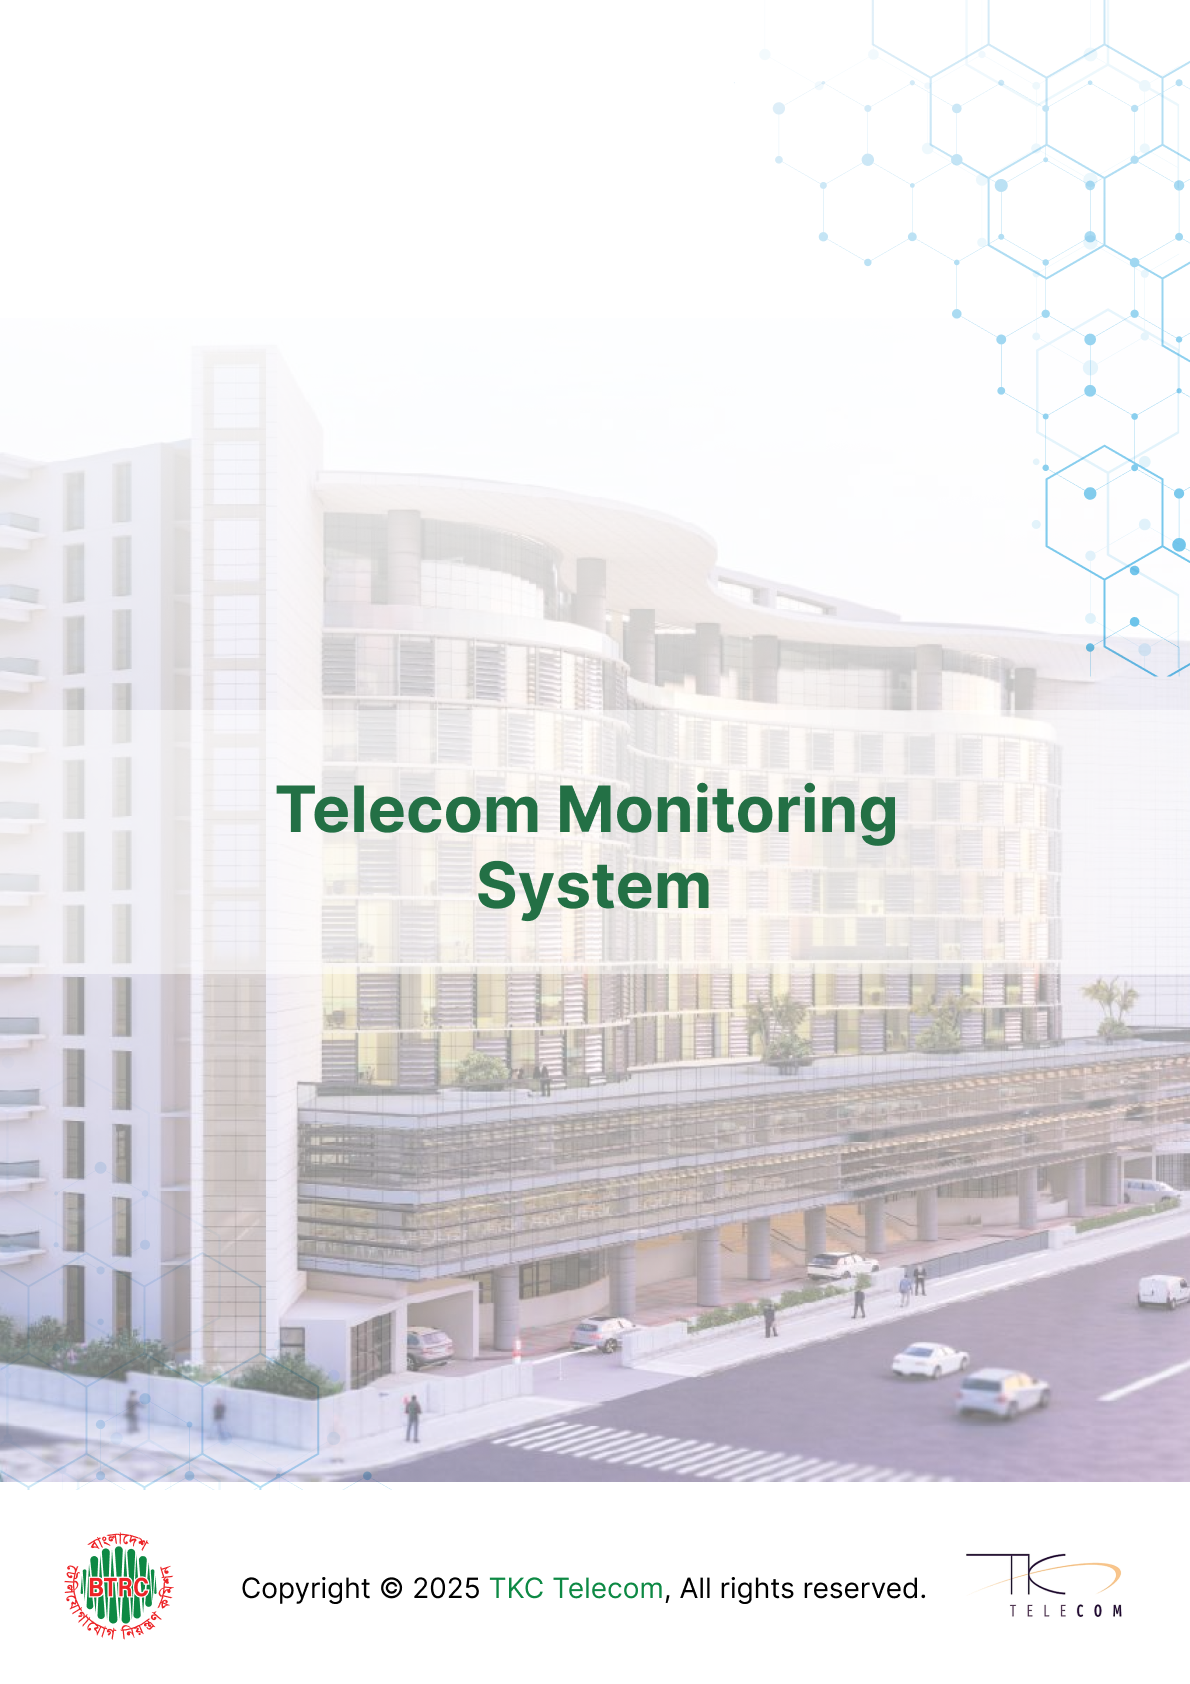
\includegraphics[width=\paperwidth,height=\paperheight]{img/common/Back.png}%
  }%
}

% Empty page content (just to ship the page)
\null
\clearpage
\end{document}